\documentclass[10pt,twocolumn,letterpaper]{article}

\usepackage{cvpr}
\usepackage{times}
\usepackage{epsfig}
\usepackage{graphicx}
\usepackage{amsmath}
\usepackage{amssymb}
\usepackage{textcomp}

% Include other packages here, before hyperref.

% If you comment hyperref and then uncomment it, you should delete
% egpaper.aux before re-running latex.  (Or just hit 'q' on the first latex
% run, let it finish, and you should be clear).
\usepackage[pagebackref=true,breaklinks=true,letterpaper=true,colorlinks,bookmarks=false]{hyperref}

\cvprfinalcopy % *** Uncomment this line for the final submission

\def\cvprPaperID{****} % *** Enter the 3DV Paper ID here
\def\httilde{\mbox{\tt\raisebox{-.5ex}{\symbol{126}}}}

% Pages are numbered in submission mode, and unnumbered in camera-ready
%\ifcvprfinal\pagestyle{empty}\fi
\setcounter{page}{1}
\begin{document}

%%%%%%%%% TITLE
\title{Image Reconstruction from DVS\\ The constant battle agains MATLAB\\ Student Project Report}

\author{Samuel Bryner\\
ETH Zurich\\
%Institution1 address\\
{\tt\small samuelbryner@student.ethz.ch}
% For a paper whose authors are all at the same institution,
% omit the following lines up until the closing ``}''.
% Additional authors and addresses can be added with ``\and'',
% just like the second author.
% To save space, use either the email address or home page, not both
\and
Marcel Geppert\\
ETH Zurich\\
%First line of institution2 address\\
{\tt\small mgeppert@student.ethz.ch}
}

\maketitle
%\thispagestyle{empty}

%%%%%%%%% ABSTRACT
\begin{abstract}

// TODO - insert abstract

\end{abstract}

%%%%%%%%% BODY TEXT
\section{Introduction}

// TODO - insert introduction here

%-------------------------------------------------------------------------
\section{Related Work}

Computer vision using dynamic vision sensors is a very young field since the
sensors have only been around for a few years \cite{lpd08dvs, brandli14davis}.
While the problem of visual odometry and visual SLAM has been known for many
years and many approaches have been proposed, the work by Kim \etal
\cite{kim2014simultaneous}, which is the basis of our work, is, to our best
knowledge, the first approach to the problem using only a DVS with no
additional information.  It has, however, already been shown that the precision
of a visual odometry system using a standard camera can be increased by adding
a DVS, especially during fast turns when the standard camera suffers from
motion blur \cite{censi13dvsd_sub}.  Additionally, DVS's have been shown to
outperform standard cameras at pose tracking during high-speed maneuvers when
used in sufficiently equipped environments \cite{mueggler2014event}.  Other
research with DVS's focuses in great parts on tracking moving objects with a
static camera \cite{vmv.20141280, conradt2009embedded, censi13led}.


\section{Dynamic Vision Sensors}

A Dynamic Vision Sensor (DVS) \cite{lpd08dvs}, also known as an event camera,
is a new kind of camera. In contrast to a standard camera it does not output a
complete image of the scene, but a series of events. An event is generated when
the sensed brightness of a pixel changes more than a certain threshold. This
happens for each pixel completely independent from all the others.

A DVS has several advantages compared to standard cameras. Since there is no
need to gather data from all pixels to generate an image, events can be sent
with an extremely low latency of $15 \mu s$ or less \cite{brandli14davis, lpd08dvs} and
with microsecond timestamps.  For the same reason, there is practically no
motion blur in the DVS signal.  Another benefit of independent pixels is the
very high dynamic range.  Saturation, blooming or smearing as observed when a
bright light source is captured with a standard camera is basically
nonexistent. Finally, due to the reduction of the camera signal to changes and
the resulting elimination of redundant temporal information, the signal
bandwidth is much smaller than with a standard camera.
All these features make the DVS a very desirable sensor for motion tracking,
especially for mobile robots where the data has to be analyzed on constrained
hardware.

However, there are currently several caveats: First of all, currently available
DVS (DVS128 \cite{lpd08dvs}, DAVIS \cite{brandli14davis}) have a very limited
resolution of $128 \times 128$ or $240 \times 180$ pixels, respectively. This
obviously limits the spacial accuracy of the sensed data, but it is likely to
be a simple matter of time until sensors with a higher resolution are
developed. A more important point is that the computer vision algorithms that
have been developed during the last decades either cannot be used at all or
have to be adapted to the new data representation.


\section{Our Work}

// TODO - insert section to explain what we did here

-implemented paper (kim) in matlab\\
-some simplifications\\
	-use particle filter directly with euler angles (ignore corner cases)\\
	-start with first fov in map\\
	
\section{Core Algorithm}
Similar to most SLAM algorithms, an iteration of our algorithm consists of two steps. In the first step we try to estimate the current orientation based on the camera signal, our map of the environment and the previous orientation. This is then used to write the new data to the map and reconstruct a grayscale image. This iteration is performed every time an event arrives from the camera. Both the tracking and the rotation work on the assumption that the output  of the other one is correct.


\subsection{Rotation Tracking}
In order to integrate intensity change events into a full gradient map of the
environment, we must track the current position and movement direction of the
camera.

The camera's position is represented using a particle filter, where each
particle consists only of a weight and the three Euler angles necessary to
describe the camera's orientation.

Whenever a new event is received, we disturb the particles randomly with
variance proportional to the time since the last event. This is essentially a
constant position model, where the camera is assumed to stay stationary between
events but with uncertainty growing with time.

To update the weights of the disturbed particles, we retrieve the position of
the camera at the time of the last event of the \textit{same} pixel (which can be a
lot earlier than the previous event). We then sample our map (from the
reconstruction part and which we assume is essentially correct) at this earlier
position. This intensity is then compared with the intensities at all the
proposed current positions: The closer the intensity difference to the
intensity threshold that generates an event, the liklier is the new position
and the more weight this particle gets.

Finally, the particles are resampled whenever the effective number of particles
(one over sum of squared weights, see \cite{kim2014simultaneous} for details)
falls below some threshold (usally $N/2$ as in \cite{kim2014simultaneous}).
Resampling is done by copying particles with probability equal to their weight
into a new set.

\subsubsection{on the matter of prior positions and accuracy}

A particle filter is a nice way of keeping track of multiple hypotheses as
might conceivably occur when updating on a single event: An event might match
multiple edges and we might only be able to resolve the correct position after
receiving further events.

But as described above, we need to know the position at the time of the
previous event of the same pixel. And as the pixels are independent, we would
have to keep a full copy of the particle filter for every pixel. This not only
requires a lot of memory, it also considerably slows down measurement updates
as we now have to compare each of the current particles with all possible
previous ones.

However, our experiments show that it is actually enough to only keep the
weighted average over the particles as any errors are quickly averaged out by
the sheer number of events.


\subsection{Scene Reconstruction}
We use Kalman Filters to reconstruct the grayscale image from the noisy DVS signal. For each pixel in the output image there is a Kalman Filter that keeps track of the color gradient at the pixel position. The input to the Kalman Filter is the event frequency on a line along the current pixel movement. Hereby it is assumed that the pixel's movement was constant since the last event it triggered. While this is obviously not true all the time, it is a good approximation due to the high rate of events. Note that the pixel movement is not necessarily parallel to the camera movement, e.g. if the camera is rotating around its z-axis.
The pixel movement is computed with the same formulas as used in the simulationand the map lookup during tracking. Given a camera orientation, the orientation of the ray through the pixel and the camera's focal point is computed. This is then mapped to a pixel in the output image. While we use the exact position in the output image to compute the pixel movement,  we do not, however, interpolate between several pixels when writing the signal to the map, but simply round the position in the output image th the closest pixel. Since we do not write the signal directly but use Kalman Filters to reduce the noise, this simplification greatly reduces the complexity of the algorithm compared to dividing the signals between several filters.
The exact formulas used for the Kalman Filters can be seen in \cite{kim2014simultaneous}.
In the current state of our program, we assume that the camera's initial field of view is already known and included in the map. With this assumption we do not have to deal with a special initialization procedure but can immediately start with the standard iteration while being relatively sure that the camera movement is tracked correctly.


\section{Problems}
// TODO - insert section about problems

-map initialization\\
-runtime\\
$\rightarrow$ couldn't test with camera\\
-MATLAB\\


\section{Experiments}
// TODO - insert section about experiments

\begin{itemize}
\item initialization
\begin{itemize}
\item integrate while removing shutter
\item integrate over short interval ($\rightarrow$ outlines)
\end{itemize}
\item camera calibration
\end{itemize}

Most of our experiments are based on the simulation described in section
\ref{sec:simulation} as our code is not performant enough to handle the amount
of events a real dynamic vision sensor generates and because the simulation
makes comparisons with ground truth much easier.
For the evaluation of the algorithm we simply simulated different camera paths
and ran the reconstruction on the generated data.
Additionally, both the tracking and the reconstruction were evaluated separately
by performing the above experiments and replacing the output of the respective
other part with ground truth data.
In preparation for a usage with real camera data, we performed two additional
experiments to evaluate the feasibility of two ideas that could be used to adapt
the algorithm to the camera data:
A method to generate an image that can be used to initialize the map and a method
to calibrate the camera using a standard camera calibration toolbox.

\subsection{Initialization by Removing Shutter}
\label{sec:shutter_removal}

If the DVS is fully covered by a shutter we can recover a full picture by
simply removing it slowly and integrating all the events generated. This allows
for an easy initialization of the map using only a basic DVS. An example is shown in figure \ref{fig:shutter_integration}.

\subsection{Camera Calibration}
\label{sec:camera_calibration}

As with any sensor, we must calibrate the DVS to get usable data. For normal
cameras, this is usually done by capturing images of a checkerboard pattern from
different viewpoints and subsequently rectifying images so they fit into a
standard pinhole camera model.

Unfortunately, the dynamic vision sensor only detects changes and cannot
directly capture a calibration pattern. We could take pictures as described in
the previous section, but for calibration \cite{mueggler2014event} proposed a different method:
Use a computer screen to quickly show and hide the pattern. With this method,
calibrating the DVS should be almost as convenient as with any standard camera.
This method can also be used to focus the camera optics by displaying a pattern
of lines with varying sizes and observing the resulting camera signal with jAER.


\subsection{Camera Simulation}
The simulation starts off with a normal image containing a 360\textdegree{}
panorama. The field of view of the camera is computed given its orientation
(normal Euler angles) and the actual camera image is created by sampling the
panorama image (the ground truth map) using raycasting. The camera is then
rotated by a tiny amount to get a second image patch. These patches are then
subtracted to get a list of events where the difference exceeds a threshold. To
also detect changes with a small absolute gradient, differences are accumulated
over time as it would happen with the real DVS. See figure \ref{fig:simulation}
for an example output.

This discrete approach is fairly straightforward but suffers from the problem
that it is very slow, as extremely tiny steps have to be taken to get accurate
events.

\begin{figure}
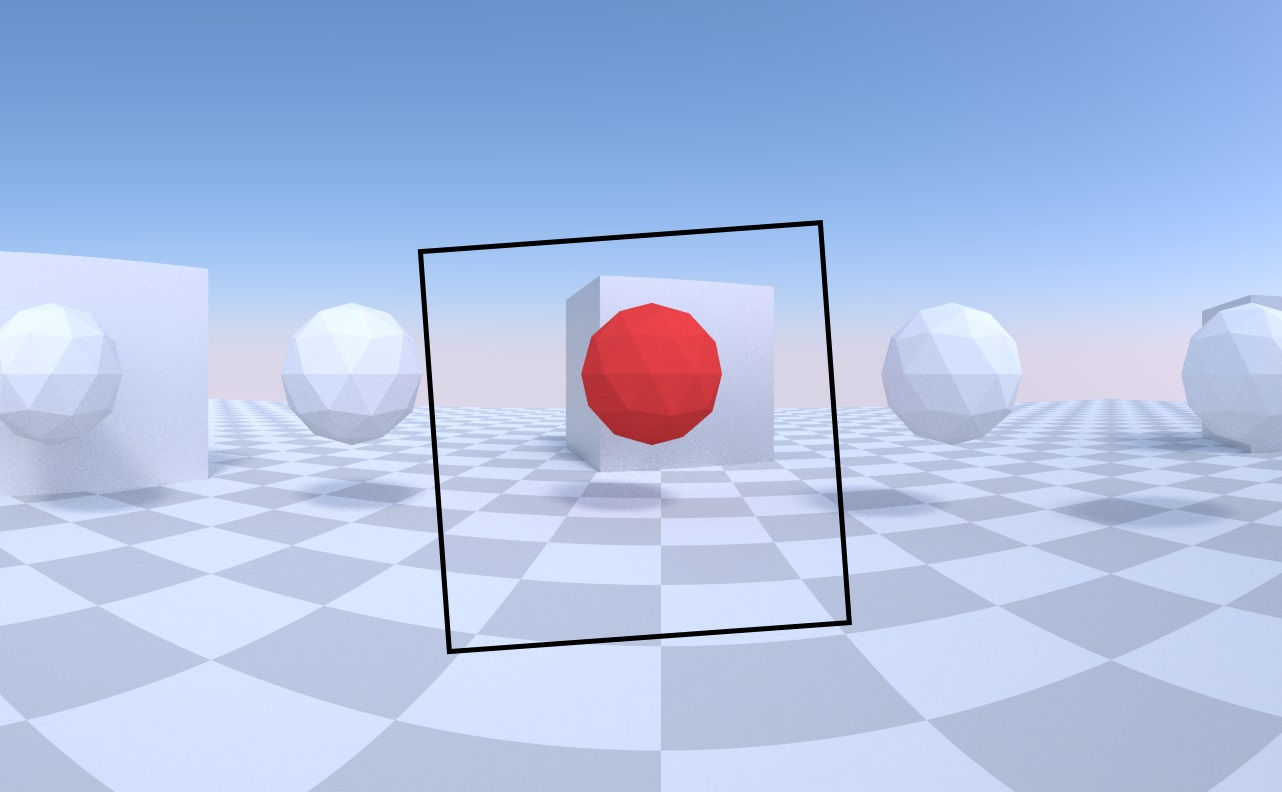
\includegraphics[width=\linewidth]{images/simulation_raw.jpg}
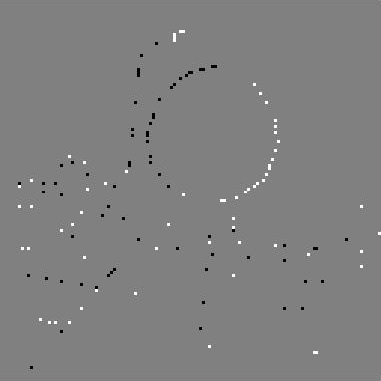
\includegraphics[width=\linewidth]{images/simulation_events.jpg}
\caption{above: the map used as input with the camera's FOV, below: events generated by moving the camera to the right}
\label{fig:simulation}
\end{figure}


\section{Results}
TODO: write some text here. Conclusion and stuff.

- influence of the various parameters
- code too slow for realtime, but not optimized at all
- using Matlab for more than just a few hacked scripts: bad idea

\begin{figure}
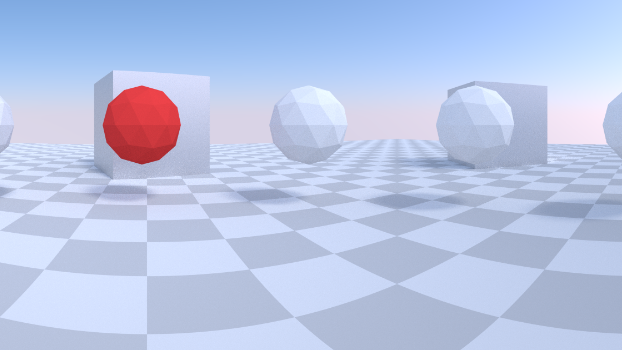
\includegraphics[width=\columnwidth]{images/zigzag_input.png}
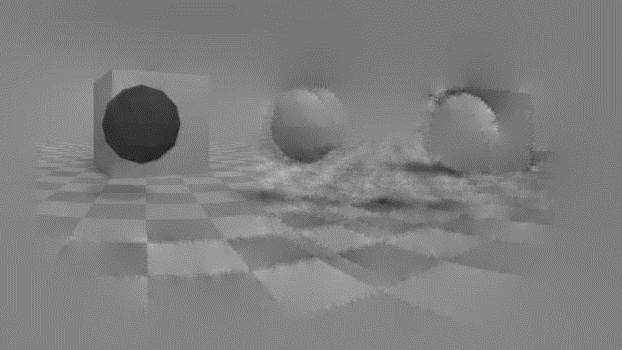
\includegraphics[width=\columnwidth]{images/zigzag_reconstruction.png}
\caption{A part of the input scene (top) and its reconstruction,
moving the camera in a large triangle waveform pattern to the right.
The area around the leftmost ball in the scene was used to initialize
the map as described in section \ref{sec:core_algorithm}.}
\label{fig:zigzag_reconstruction}
\end{figure}



{\small
\bibliographystyle{ieee}
\bibliography{references}
}

\end{document}
